\documentclass{article}
\usepackage{graphicx}
\usepackage{booktabs}
\usepackage{geometry}
\usepackage{tikz}
\usetikzlibrary{shapes, arrows.meta, positioning, backgrounds, fit}

\geometry{a4paper, margin=1in}

\title{Intelligent EV Charging Demand Prediction \\ \large Milestone 1: Model Evaluation \& System Architecture}
\author{Project 15}
\date{February 16, 2026}

\begin{document}

\maketitle

\section{Executive Summary}
This report analyzes the performance of the Machine Learning model developed to predict EV charging station utilization rates. The model uses historical usage data along with temporal, environmental, and traffic features to forecast demand.

\textbf{Key Results:}
\begin{itemize}
    \item \textbf{R-Squared ($R^2$):} 0.9045 (Excellent predictive power)
    \item \textbf{RMSE:} 0.0926 (Low average error magnitude)
    \item \textbf{MAE:} 0.0634 (Very low absolute error)
\end{itemize}

The model demonstrates strong capability in conducting accurate demand forecasting, suitable for infrastructure planning and real-time user insights.

\section{System Architecture}

\begin{figure}[h]
    \centering
    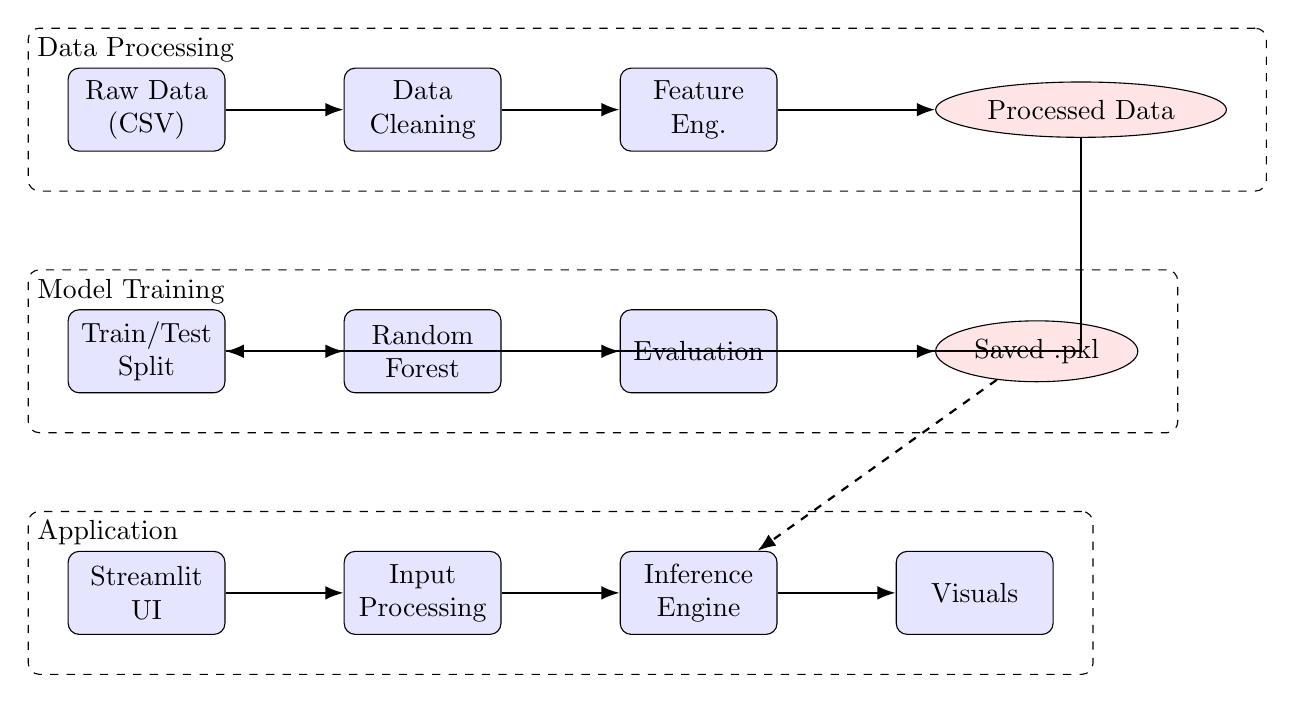
\begin{tikzpicture}[
        node distance=1.5cm,
        auto,
        block/.style={rectangle, draw, fill=blue!10, text width=5em, text centered, rounded corners, minimum height=3em},
        cloud/.style={draw, ellipse, fill=red!10, node distance=2cm, minimum height=2em},
        decision/.style={diamond, draw, fill=green!10, text width=4.5em, text bad centered, inner sep=0pt},
        line/.style={draw, -Latex, thick},
        container/.style={draw, dashed, inner sep=0.5cm, rounded corners, label={[anchor=north west]north west:#1}}
    ]
        % Data Layer
        \node [block] (raw) {Raw Data (CSV)};
        \node [block, right=of raw] (clean) {Data Cleaning};
        \node [block, right=of clean] (feat) {Feature Eng.};
        \node [cloud, right=of feat] (processed) {Processed Data};
        
        \path [line] (raw) -- (clean);
        \path [line] (clean) -- (feat);
        \path [line] (feat) -- (processed);
        
        \begin{scope}[on background layer]
            \node [container=Data Processing, fit=(raw) (processed)] (data_layer) {};
        \end{scope}

        % Model Layer
        \node [block, below=2cm of raw] (split) {Train/Test Split};
        \node [block, right=of split] (rf) {Random Forest};
        \node [block, right=of rf] (eval) {Evaluation};
        \node [cloud, right=of eval] (model) {Saved .pkl};

        \path [line] (processed) |- (split); % Link from Data to Model
        \path [line] (split) -- (rf);
        \path [line] (rf) -- (eval);
        \path [line] (eval) -- (model);
        
        \begin{scope}[on background layer]
            \node [container=Model Training, fit=(split) (model)] (model_layer) {};
        \end{scope}

        % Application Layer
        \node [block, below=2cm of split] (ui) {Streamlit UI};
        \node [block, right=of ui] (input) {Input Processing};
        \node [block, right=of input] (infer) {Inference Engine};
        \node [block, right=of infer] (viz) {Visuals};

        \path [line] (ui) -- (input);
        \path [line] (input) -- (infer);
        \path [line] (infer) -- (viz);
        \path [line, dashed] (model) -- (infer); % Link from Model to App

        \begin{scope}[on background layer]
            \node [container=Application, fit=(ui) (viz)] (app_layer) {};
        \end{scope}

    \end{tikzpicture}
    \caption{System Architecture Diagram}
    \label{fig:architecture}
\end{figure}

\section{Model Specification}
\begin{itemize}
    \item \textbf{Algorithm:} Random Forest Regressor
    \item \textbf{Framework:} Scikit-Learn (Pipeline with ColumnTransformer)
    \item \textbf{Input Features:}
    \begin{itemize}
        \item \textbf{Temporal:} Hour of Day, Day of Week, Is Weekend, Is Peak Hour
        \item \textbf{Environmental:} Temperature (°F), Precipitation (mm), Weather Category
        \item \textbf{Contextual:} Traffic Congestion Index, Gas Price, Local Events
        \item \textbf{Station:} Location Type, Charger Type, City
    \end{itemize}
\end{itemize}

\section{Detailed Performance Metrics}

\begin{table}[h]
    \centering
    \begin{tabular}{@{}llp{8cm}@{}}
        \toprule
        \textbf{Metric} & \textbf{Value} & \textbf{Interpretation} \\
        \midrule
        R-Squared ($R^2$) & 0.9045 & The model explains \textbf{90.45\%} of the variance in charging demand. Indicates high fit to real-world patterns. \\
        RMSE & 0.0926 & On average, predictions deviate by \textbf{9.3\%} from actual utilization. \\
        MAE & 0.0634 & The average absolute difference between predicted and actual utilization is \textbf{6.3\%}. \\
        \bottomrule
    \end{tabular}
    \caption{Model Evaluation Metrics}
    \label{tab:metrics}
\end{table}

\section{Conclusion}
The Random Forest model satisfies the technical requirements for Milestone 1, achieving high accuracy without reliance on deep learning or agentic methods. It is robust enough for deployment in the interactive Streamlit dashboard.

\end{document}
